% Created 2020-01-10 Fri 15:48
% Intended LaTeX compiler: pdflatex
\documentclass[a4paper, dvipdfmx, 10pt]{article}
\usepackage[utf8]{inputenc}
\usepackage[T1]{fontenc}
\usepackage{graphicx}
\usepackage{grffile}
\usepackage{longtable}
\usepackage{wrapfig}
\usepackage{rotating}
\usepackage[normalem]{ulem}
\usepackage{amsmath}
\usepackage{textcomp}
\usepackage{amssymb}
\usepackage{capt-of}
\usepackage{hyperref}
\usepackage{minted}
\usepackage{amsmath, amssymb, bm}
\usepackage{graphics}
\usepackage{color}
\usepackage{times}
\usepackage{longtable}
\usepackage{minted}
\usepackage{fancyvrb}
\usepackage{indentfirst}
\usepackage{pxjahyper}
\usepackage[utf8]{inputenc}
\usepackage[backend=biber, bibencoding=utf8]{biblatex}
\usepackage[top=20truemm, bottom=25truemm, left=25truemm, right=25truemm]{geometry}
\hypersetup{colorlinks=false, pdfborder={0 0 0}}
\usepackage{ascmac}
\usepackage{algorithm}
\usepackage{algorithmic}
\addbibresource{./qareport.bib}
\author{MokkeMeguru}
\date{\textit{<2019-04-24 Wed>}}
\title{強力なNormalization手法、GauGAN (SPADE) を読む}
\begin{document}

\maketitle
\tableofcontents


\section{導入}
\label{sec:org5eb6cd0}
GauGAN [1] というのは 2019 年画像生成系の分野を賑わせた新たな Normalization (正規化) 手法についての論文で、NVIDIAの研究成果になります。website [2] でそのデモを体験することが出来、日本でも深層学習をやっている人たちが盛り上がっていたイメージです。\\
あと \textbf{\textbf{実装が PyTorch なので}} 大変読みやすく、バグがないです。\\
\begin{center}
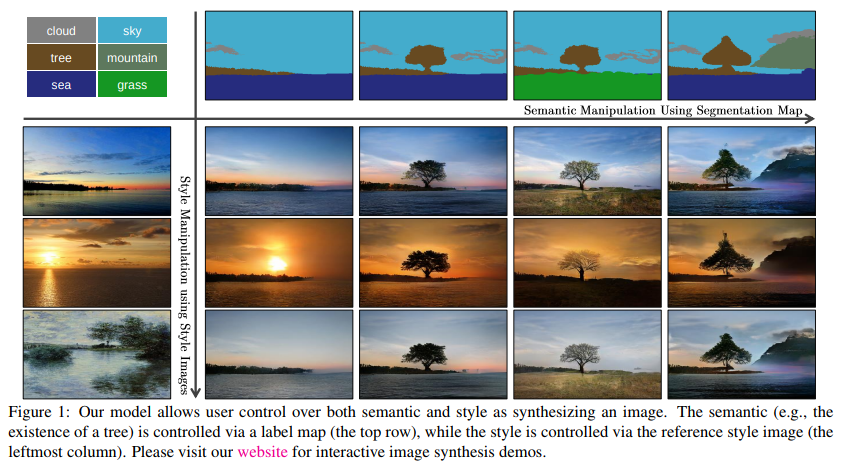
\includegraphics[width=18cm]{./gaugan_image.png}
\end{center}

[1]: \href{https://arxiv.org/abs/1903.07291}{Semantic Image Synthesis with Spatially-Adaptive Normalization}\\

[2]: \href{https://github.com/NVlabs/SPADE}{Github}\\

\section{GauGAN の取り組む問題}
\label{sec:org793417e}
GauGAN が取り組むタスクは Semantic Image Synthesis というものです。こは簡単に言ってしまうと \textbf{\textbf{こんな感じの画像を作りたい}} というイメージから \textbf{\textbf{写真のような画像}} を生成することを指し、パッとWebの背景画像を作りたいとか、ゲームの画像を作りたいとかいった場面で役に立ちます。\\

本研究の Semantice Image Synthesis において、入力は概形を描いたセグメンテーション画像 (色分けした画像) であり、出力は写真のような画像、となっています。関連研究としては、例えば入力が単語であったりする場合があります。\\

本研究で用いたデータセットの一つとして \href{https://github.com/nightrome/cocostuff}{COCO-Stuff dataset} があります。これは写真データと、そのセグメンテーション画像がペアになっています。本来的には COCO-Stuff は写真データ -> セグメンテーション画像、というふうな学習を目的としたデータセットなのですが、本研究ではその逆を行なっている点に注意して下さい。\\

\begin{center}
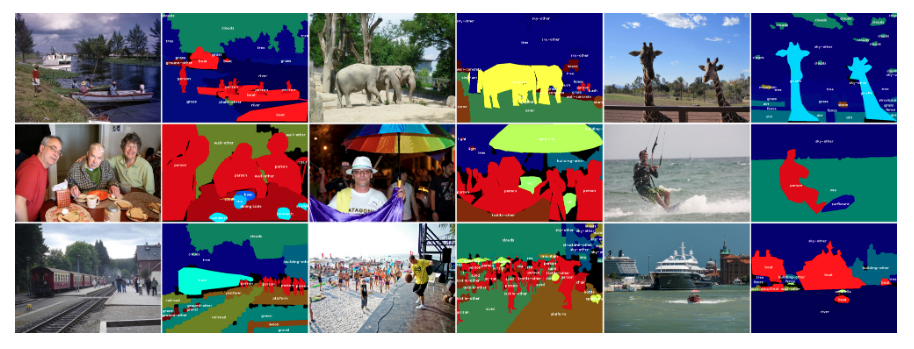
\includegraphics[width=18cm]{./coco.png}
\end{center}

\section{Normalization とは何か}
\label{sec:org6825574}
Normalization (正規化) とは雑に言うと \(\bm{x}\) の値域を \(\bm{x'}\) へ変換することを指します。 \textbf{\textbf{変換前後の次元的に言うと、 \(f: \mathbb{R}^{H \times W \times C} \rightarrow \mathbb{R}^{H \times W \times C}\) です}} 。\\
画像データ \(\mathbb{R}^{N \times H \times W \times C}\) (\(N\) : バッチサイズ、 \(H\) : 画像の高さ、 \(W\) : 画像の幅、 \(C\) : 画像のチャンネル ) を例にすると、次のようなものが例として挙げることが出来ます。\\
\begin{itemize}
\item BatchNormalization\\

\(C\)  について \(\mu = 0\) ,  \(\sigma = 1\) への正規化をします。このとき平均・分散の求め方は \(\mu_B = \cfrac{1}{N  H  W}\Sigma X_{n, h, w}\) \(\sigma^2_B = \cfrac{1}{N  H  W}\Sigma (X_{n, h, w} - \bar{X)}^2 \in \mathbb{R}^{C}\)  のようになります。(バッチサイズ \(N\) が存在していることに注意)\\

正規化の式について簡単に取り上げると、一枚画像 \(x\) の \(C\) 軸について \(\hat{x_i} = \cfrac{1}{\sigma_B}(x_i- \mu_B), x_i \in \mathbb{R}^{C}\) となります。(但し実装や性能向上のために、実際はもっと複雑な式が用いられます。)\\
\end{itemize}
\begin{itemize}
\item InstanceNormalization\\

\(C\) について  \(\mu = 0\) ,  \(\sigma = 1\) への正規化をします。但しこのときの平均・分散の求め方は \(\mu_I = \cfrac{1}{HW}\Sigma x_{h, w}\) \(\sigma^2_I  = \cfrac{1}{HW} \Sigma (x_{h, w} - \bar{x})^2\) のようになります。Batch Normalization が画像データ群全体で \(C\) が \(\mu=0, \sigma^2=1\) となるようにしているのに対して Instance Normalization が 一枚の画像について \(\mu=0, \sigma^2=1\) に正規化している点が主な違いです。\\
\item ActNorm\\

ActNorm は Glow[3] で提案された Normalization で、これは \textbf{\textbf{まず}} 初期バッチ \(X_B = {x_1, x_2, ..., x_n}\) について、次の式に従うようにして \(C\) について  \(\mu = 0\) ,  \(\sigma = 1\) への正規化を行います。\\

\(\mu_{init} = \cfrac{1}{NHW} \Sigma X_{n, h, w}, \sigma^2_{init} = \cfrac{1}{NHW} \Sigma (X_{n, h,w} - \bar{X})^2 \in \mathbb{R}^{C}\)\\

ActNorm の \(\mu_{init}, \sigma^2_{init}\)  は、初期バッチで初期化された後、特に \(C\) について正則化をするという制約をかけられず、ただの訓練パラメータとして用いられます。つまりこの Normalization は \(\mu = 0\) ,  \(\sigma = 1\) への変換ではないという点に注意して下さい。\\
\end{itemize}

\begin{center}
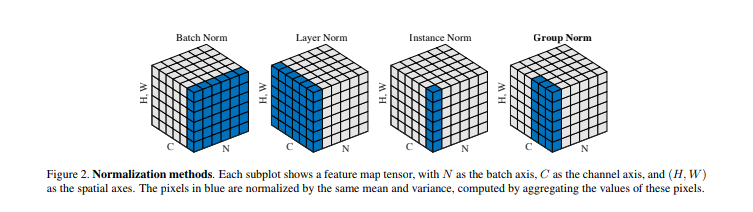
\includegraphics[width=15cm]{./normalization.png}
\end{center}

正規化について直感的な図を Group Normalization [4] から引用しましょう。例えば BatchNormalization の場合、青い部分がシュッとなって \(\mu_{B_i}, \sigma^2_{B_i}\) となります。これが \(C\) 個出来るので、 \(\mu_B \in \mathbb{R}^{C}\) です。Instance Normalization は同様に考えると \(\mathbb{R}^{C B}\) ですが、バッチ軸についてはまとめ上げられるので \(\mathbb{R}^{C}\) となります。\\


[3]: \href{https://arxiv.org/abs/1807.03039}{Glow: Generative Flow with Invertible 1x1 Convolutions}\\

[4]: \href{https://arxiv.org/pdf/1803.08494.pdf}{Group Normalization}\\
\section{SPADE (Spatially-Adaptive (DE)normalization)}
\label{sec:org3ecf2a4}
GauGANでは Normalization について新たな手法 SPADE (Spatially-Adaptive (DE)normalization) を提案しました。\\
  特にこの Normalization は Conditional Normalization の一種としてみなされます。Conditional Normalization の関連手法としては Conditional Batch Normalization や AdaIN を挙げることが出来ます。これらは外部のデータを用いた手法であり、この手順は (1)  BatchNormalization などの手法で 平均 0, 分散 1 へ正規化を行い \(x\) を獲得 、(2) 外部のデータを用いてアフィン変換 \(ax + b\) を行う、というものになっています。先行研究でのアフィン変換のパラメータ \(a, b\) はベクトルであったりスカラーであったりいろいろですが、SPADE ではここにセグメンテーション画像を用いました。\\
\subsection{SPADE のコンセプト}
\label{sec:org3f80a68}
\begin{quote}
their normalization layers tend to “wash away” information contained in the input semantic masks.\\
--- quoted from page 2 line 1\\
\end{quote}

SPADEのコンセプトは、 \textbf{\textbf{BatchNormalization らが "wash away(洗い流す)"  する内容を復元する}} ということです。そして彼らは復元する情報源として \textbf{\textbf{セグメンテーション画像}} を使いました。\\

直感的な説明をしましょう。例えばセグメンテーション画像からハワイの海岸の画像を生成しようとするとき、海の部分と砂浜の部分を同じように平均 0,  分散 1 にされてしまうと (ここで Batch Normalization が \(C\) について正規化されているという点を思い出してみましょう) 情報落ちてない?となるわけです。ここで Conditional Normalization をして情報補完をしてみよう→どうやって補完する?→そういえばセグメンテーション画像なんてものがあるな、みたいな感じに発想を進めていくことが出来ます(いや彼らがそう思っているかは知りませんが)。\\

下の画像が SPADE のレイヤーの概要です。確かに (1) BatchNormalization (2) セグメンテーション画像から \(\gamma, \beta\) を用いてアフィン変換、をしていますね。\\
\begin{center}
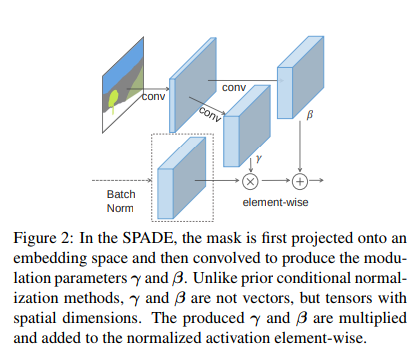
\includegraphics[width=10cm]{./spade_abst.png}
\end{center}

\subsection{SPADE の細かい話}
\label{sec:org1c6efb8}
次に細かい話としてSPADE の入力と出力を示しましょう。前提として、SPADE は BatchNormalization に合わせて モデルの複数ヶ所に適用されるので、それぞれの SPADE を \(i\) で区別します。\\

SPADEの入力はセグメンテーション画像で、セグメンテーションラベルは \href{https://github.com/NVlabs/SPADE/issues/29}{one-hot vector になっており} 、 つまりこれがいわゆるセグメンテーション画像の \(C\) になります。これが \(H^{i} \times W^{i}\) 個あるので、結局 SPADE の入力は \(m\in (\mathbb{L}^{H^{i}\times W^{i}} = \mathbb{R}^{H^{i} \times W^{i} \times {C^{i}}'})\) となります。 \(\beta^{i}, \gamma^{i}\) をそれぞれ後述する式で求めます。\\
それはそれとして、BatchNormalization Layer から \(\mu^{i}, \sigma^{i}\) をそれぞれ用意しておきます。\\

BatchNormalization Layer に入ってくる Tensor \(h^{i}\) と \(\mu^{i}, \sigma^{i}, \beta^{i}, \gamma^{i}\) から \(h^{i}\) -> [BN -> SPADE] -> \({h^i}'\) は 次の式で表すことが出来ます。\\

\begin{eqnarray*}
{h^i}' = \gamma^i \cfrac{h^{i} - \mu^{i}}{\sigma^{i}} + \beta^{i}
\end{eqnarray*}

ここであれ?って思える人は深層学習の実装に向いています。そう、この式ですと次元数があんまりよくわかんないです。なので、詳しく次元数を書いてみます。\\

\begin{eqnarray*}
, where\\
h^{i} &\in& \mathbb{R}^{N \times H^{i} \times W^{i} \times C^{i}}\\ 
\mu^{i}, \sigma^{i} &\in& \mathbb{R}^{C^{i}} \\
 \gamma^{i}, \beta^{i} &\in& \mathbb{R}^{H^{i} \times W^{i} \times C^{i}}
\end{eqnarray*}

つまり Batch Normalization が \(C^{i}\) について正規化が行われているのに対して、SPADE は \(H^{i}, W^{i}, C^{i}\) について正規化が行われています。\\

雑な発想ですと、セグメンテーション画像をそのままペッと \(\cfrac{h^{i}-\mu^{i}}{\sigma^i}\) へ貼っているイメージでしょうか。こうすることで Batch Normalization で落としてしまったであろう情報を復元できるというわけです。\\
\section{モデルの全容}
\label{sec:org07a6aa4}
本研究で特にセグメンテーション画像を使っている部分は一般的なGANs でいう Generator と Discriminator の部分なので、これらについて概形→詳細、と詰めて見てみましょう。\\

\begin{center}
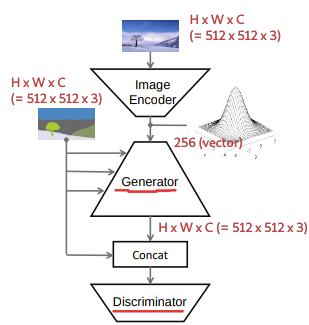
\includegraphics[width=10cm]{./gaugan_full.png}
\end{center}

\subsection{Generator}
\label{sec:org8a48ba0}
最終的な出力が \(N \times H \times W \times C = 256 \times 512 \times 512 \times 3\) の画像となる Generator を下に引用します。\\

\texttt{SPADE ResBlk(K)} は入力を \(N \times H^{i} \times W^{i} \times C^{i}\) の入力を受け取り \(N \times H^{i} \times W^{i} \times K\) を出力します。そして \texttt{Upsample(2)} は \(N\times H^{i} \times W^{i} \times K\) を入力として \(N \times 2H^{i} \times 2W^{i}  \times K\) を出力とします。例として、上から1つ目の  \texttt{SPADE ResBlk(1024), Upsample(2)} は、 \(N \times 4 \times 4 \times 1024\) を入力として \(N \times 8 \times 8 \times 1024\) を出力とします。(以降バッチサイズ \(N\) を省略)\\
\begin{center}
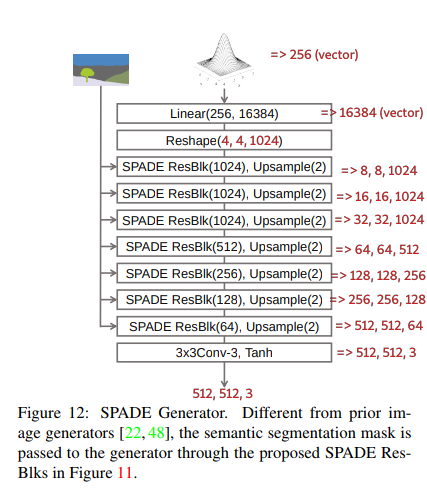
\includegraphics[width=10cm]{./gaugan_gen.png}
\end{center}
\subsubsection{SPADE ResBlk}
\label{sec:orge746ca6}
SPADE ResBlk については、下に引用される図で説明します。ResNet を元にしていますが、入力と出力の次元数が異なっている点に注意して下さい。簡単な構造は ResNet と変わっていませんが、正規化層がそのまま SPADE に置き換わっており、SPADEのための入力であるセグメンテーション画像が外部から与えられていることがわかると思います。\\
   \texttt{SxSConv-K} は カーネルサイズ \(S\) フィルタサイズ \(K\) の畳み込みを示しており、\(H\times W\times C\) のTensorを入力として \(H \times W \times K\) の Tensor を出力とします。\\
\begin{center}
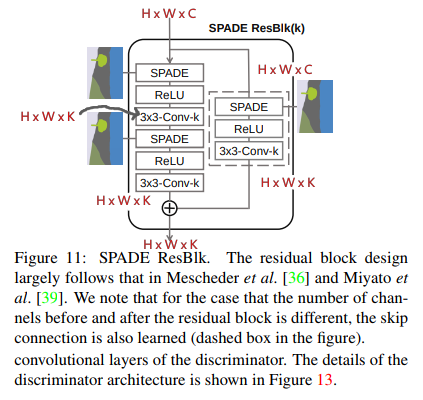
\includegraphics[width=10cm]{./SPADE_ResBlk.png}
\end{center}

\subsubsection{SPADE}
\label{sec:org1514483}
SPADE そのものについては、下に引用される図で説明します。ここで注意してほしいのは、SPADEそのものは \textbf{\textbf{入力と出力で次元数が変わらない=通常のNormalizationと同じ}} という点です。すると問題になるのが、 \textbf{\textbf{セグメンテーション画像をどう扱うか}} です。\\
 セグメンテーション画像は一枚の \(H'\times W' \times C' = 512 \times 512 \times C'\) で共通であり、これは SPADE に入ってくるデータの次元数 \(H^{i} \times W^{i} \times C^{i}\) とは異なります。 \(C\) については畳み込みレイヤーでどうとでもなるのですが (3x3-Conv-k で変えられる) \(H, W\) についてはそうはいきません。なので SPADE では Resize を使って \(H, W\) の変換を行います。\\

\begin{center}
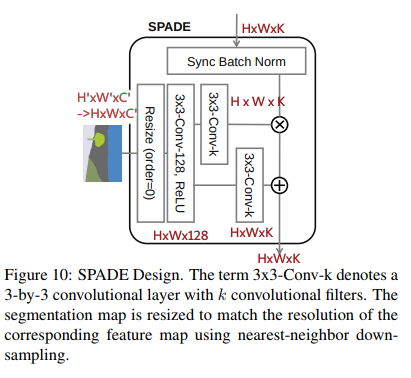
\includegraphics[width=10cm]{./spade.png}
\end{center}

\subsection{Discriminator}
\label{sec:orgace7975}
Discriminator は Pix2PixHD と同等の機能を持っています。この Discriminator の図がわかりにくいので簡単に Pix2PixHD から引用を行いながら説明を行います(というか既存の解説記事はこのあたりの話雑すぎませんか?)。\\

\begin{quote}
To address the issue, we propose using multi-scale discriminators. We use 3 discriminators that have an identical network structure but operate at different image scales.\\
We will refer to the discriminators as D1, D2 and D3. Specifically, we downsample the real and synthesized highresolution images by a factor of 2 and 4 to create an image pyramid of 3 scales. The discriminators D1, D2 and D3 are\\
then trained to differentiate real and synthesized images at the 3 different scales, respectively.\\
Although the discriminators have an identical architecture, the one that operates at the coarsest scale has the largest receptive field.\\
It has a more global view of the image and can guide the generator to generate globally consistent images. On the other hand, the discriminator at the finest scale encourages the\\
generator to produce finer details. This also makes training the coarse-to-fine generator easier, since extending a lowresolution model to a higher resolution only requires adding\\
a discriminator at the finest level, rather than retraining from scratch.\\
Without the multi-scale discriminators, we observe that many repeated patterns often appear in the generated images.\\

--- quoted from Pix2PixHD page 4 second column\\
\end{quote}
\begin{center}
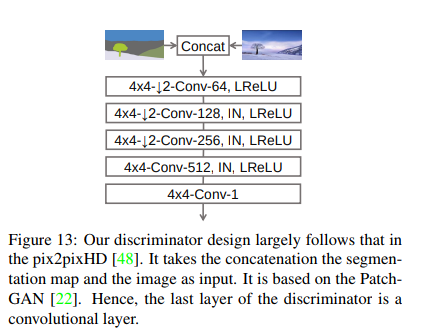
\includegraphics[width=10cm]{./gaugan_disc.png}
\end{center}
\section{訓練・推論手法}
\label{sec:org2ba1801}
\section{実験}
\label{sec:orgfb157d0}
\section{結果}
\label{sec:org2ba663c}
\section{論文のアブストラクト・イントロダクションの和意訳}
\label{sec:org1d2865c}
アブストラクト\\
\section{読んだ感想とか}
\label{sec:orgaf1a5bc}
\end{document}
